\documentclass[]{ceurart}

\sloppy

%% Math + tables + graphics used by the body (ceurart already loads
%% amsmath/graphicx/natbib, but we load the extras the body needs).
\usepackage{amssymb}
\usepackage{amsthm}
\usepackage{booktabs}
\usepackage{tikz}
\usetikzlibrary{positioning, arrows.meta}
\newtheorem{proposition}{Proposition}

%% Title at \Large (not the default \LARGE) so it fits two lines.
%% Set via the class key system; a size macro inside \title{} breaks pdfx metadata.
\ExplSyntaxOn
\keys_define:nn { ceur / title } {
  mode / title .meta:n = {
    type = title, size = \Large, shape = \sffamily, weight = \bfseries,
    color = black, before = 0pt, after = 0pt, align = \raggedright,
  },
}
\ExplSyntaxOff

\begin{document}

\copyrightyear{2026}
\copyrightclause{Copyright for this paper by its authors.
  Use permitted under Creative Commons License Attribution 4.0
  International (CC BY 4.0).}

\conference{ELMKE 2026: 4th Workshop on Evaluation of Language Models in
  Knowledge Engineering, co-located with ISWC 2026, October 25--29, 2026,
  Bari, Italy}

\title{When Does Memory Help an LLM Judge? A Leakage-Free,
  Audited Evaluation of Memory-Augmented Judging}

\author[1]{Khush Patel}[%
email=k.patel@innopolis.university,
]
\cormark[1]
\author[1]{Bader Rasheed}[%
email=b.rasheed@innopolis.university,
]
\address[1]{Innopolis University, Innopolis, Russian Federation}
\cortext[1]{Corresponding author.}

\begin{abstract}
Giving an LLM judge a persistent memory of its past evaluations seems like it should help. We build such a judge and evaluate it under two protocols. Under a conventional, un-audited protocol (memory updated during evaluation, related test items not separated), memory appeared to add 6--10 accuracy points; under a careful one, no gain is detectable. The careful protocol is leakage-free (question-level data split plus frozen memory) with a two-layer audit (a SHA-256 fingerprint of the full stored graph state plus runtime write-blocking) that verifies, for every run, that memory was not modified during evaluation. Under this protocol, with GPT-4o, no memory or tree-search configuration significantly outperforms a plain stateless judge (the design is powered to detect the conventional 6--10 point claim, not few-point effects), and an apparent catastrophic collapse under memory poisoning turns out to be a harness defect, not a system property. A per-item verdict analysis explains the null: memory changes only 10\% of verdicts, and the verdicts it changes follow the judge's leniency bias rather than the ground truth. We bound the achievable benefit of memory by how far the label posterior moves once memory is revealed, plus the judge's own decision noise, characterize when memory should help, and propose practical remedies. A response-length shortcut scores 75\% on the held-out set, above every configuration tested, so absolute accuracies on this benchmark partly reflect a superficial cue. The protocol and audit are released as a reusable instrument.
\end{abstract}

\begin{keywords}
  LLM-as-a-Judge \sep
  evaluation methodology \sep
  memory-augmented evaluation \sep
  knowledge graphs \sep
  evaluation leakage \sep
  negative result
\end{keywords}

\maketitle

\section{Introduction}

LLMs now grade other LLMs. A judge model reads a task, a candidate response, and a rubric, and returns a verdict \citep{mt_bench2023, geval2023, judge_survey2024}; these verdicts rank chatbots, score agents, and feed reward signals during training, so whether the judge can be trusted matters \citep{chateval2023, llm_judge_agreement2024}.

A standard judge is stateless. It sees each item in isolation, so it cannot recognize a near-identical past case, reuse a good line of reasoning, or learn from a mistake. A natural remedy is memory: let the judge retrieve its relevant past evaluations before deciding, in the spirit of retrieval-augmented generation \citep{rag_original2020} and agent memory systems \citep{memgpt2023, generative_agents2023, reflexion2023}; evaluators that accumulate experience across sequential test items have already begun to appear \citep{jwa2026experienced}.

We built exactly this system. The complication is that memory is also a leakage channel. A store of past evaluations can propagate old errors, can be poisoned \citep{rag_poisoning2024}, and, most subtly, can carry information about a test item into the evaluation of that same item. Contamination is a known way to inflate benchmark scores \citep{data_contamination2024, benchmark_contamination2024, eval_leakage2024}, and a memory written during evaluation is a direct contamination channel. Prior memory-augmented systems assume this is not happening; none verifies it.

We verify it. Our contributions are:

\begin{enumerate}
    \item \textbf{A protocol that verifies the absence of memory mutation instead of assuming it} (\S\ref{sec:protocol}): split the benchmark by question so paired pass/fail items never straddle the split, freeze memory during evaluation, and verify the freeze with a two-layer audit (a SHA-256 fingerprint over the full stored graph state, every node's labels and properties and every edge, taken before and after evaluation, plus runtime write-blocking at both the wrapper-method and raw-Cypher level). The audit is mechanical: a hash either matches or it does not.
    \item \textbf{A corrective null result} (\S\ref{sec:results}). Under the audited protocol, none of our memory or tree-search configurations significantly beats the stateless GPT-4o judge: not with the judge's own memory, not with oracle (ground-truth) memory, not with a simpler schema, not on other random seeds. The audit also caught a real write-back leakage bug in our own evaluation path on its first run, and a corrected harness showed that an apparent collapse to 21.2\% accuracy under 50\% memory poisoning was caused by network errors being scored as wrong answers.
    \item \textbf{A mechanistic explanation of the null} (\S\ref{sec:analysis}). We read the per-item verdicts instead of stopping at aggregate accuracy. Memory leaves 90\% of verdicts unchanged, and the verdicts it does change flip mostly toward ``pass'' and are mostly wrong: the changed verdicts skew toward ``pass,'' consistent with a leniency-anchoring account rather than with memory contributing evidence, and in line with the documented sensitivity of LLMs to the content and order of in-context exemplars \citep{lu2022fantastically, zhao2021calibrate}; we treat this as a hypothesis, and the balanced-retrieval test below neither confirms nor refutes it as the cause of the null. We formalize this with a Bayes-ceiling argument: memory can raise the achievable accuracy only insofar as the conditional label distribution $P(Y\mid X,M)$ differs from $P(Y\mid X)$, which the leakage-free protocol is designed to hold close to equality, while the separate channel of stabilizing the realized (stochastic) judge has at most the judge's measured 5--10\% self-disagreement to work with. The same account predicts when memory \emph{should} help and yields concrete fixes: balanced contrastive retrieval, similarity-gated injection, and population-level calibration.
\end{enumerate}

\section{Related Work}

\paragraph{LLM-as-a-Judge.} G-Eval, MT-Bench, and Prometheus \citep{geval2023, mt_bench2023, prometheus2023} showed LLM judges can track human raters. The judges also carry position, length, and self-preference biases \citep{llm_judge_bias2024, position_bias2024}, fragile agreement, and poorly calibrated confidence \citep{chateval2023, llm_judge_agreement2024, judge_calibration2024}. Closest to our setting, \citet{jwa2026experienced} build evaluators that selectively accumulate insights while judging a test sequence, exactly the kind of cross-case learning whose evaluation our protocol is designed to keep leakage-free. The reliability of LLMs as evaluators is an active concern in knowledge engineering as well: \citet{hannah2025knowledge} use an LLM as a proxy evaluator of knowledge quality and report that it ``shows promise'' but is not yet dependable, and evaluation-quality studies of LLM-generated knowledge artefacts reach similarly cautious conclusions \citep{llugiqi2025experts, fathallah2024llms4life}. A stateless judge additionally has no way to be consistent across related items, which is the opening for memory.

\paragraph{Retrieval- and memory-augmented systems.} RAG \citep{rag_original2020} and its adaptive variants \citep{active_rag2023, self_rag2023} condition generation on retrieved evidence. Agent memory systems such as MemGPT \citep{memgpt2023}, Generative Agents \citep{generative_agents2023}, and Reflexion \citep{reflexion2023} store episodes or self-feedback for reuse. Graph-structured agent memories are likewise established, from knowledge-graph world models to agentic and temporal memory graphs \citep{anokhin2025arigraph, xu2025amem, rasmussen2025zep}, and how agents follow stored experiences, including how memory errors propagate, has been studied directly \citep{xiong2026memory}. A memory-augmented judge retrieves past evaluations as contrastive references. Our contribution is orthogonal to this line: we treat persistent memory as an evaluation-leakage surface and audit it.

\paragraph{Test-time search.} Chain-of-Thought \citep{chain_of_thought2022}, Self-Consistency \citep{self_consistency2023}, Tree of Thoughts \citep{tree_of_thoughts2023}, and ReAct \citep{react2023} spend more inference compute for better reasoning; MCTS-Judge \citep{mcts_judge2025} applies Monte Carlo Tree Search \citep{uct2006, mcts_survey2012} to judging. Our MCTS components follow this line; under the audited protocol they cost $9\times$ the latency with no significant gain, and we report them as exploratory.

\paragraph{Contamination and leakage.} Contamination inflates scores \citep{data_contamination2024, benchmark_contamination2024, eval_leakage2024}, PoisonedRAG \citep{rag_poisoning2024} corrupts outputs through small injections into a retrieval store, and agent \emph{memory} poisoning specifically has been demonstrated \citep{chen2024agentpoison, dong2025minja}. We name the two channels specific to memory-augmented judging, paired-item leakage and write-back leakage, and close both by construction, with a per-run audit.

\section{The Memory-Augmented Judge}
\label{sec:system}

\paragraph{Typed memory graph.} Memory is stored in a Neo4j property graph \citep{neo4j2023} with five node types: \textbf{Policy} (a grading rule), \textbf{Attempt} (a past response with its verdict and reasoning), \textbf{Issue} (a specific problem found), \textbf{Fix} (a correction), and \textbf{Semantic} (a category grouping similar issues), linked by four typed relations (Figure~\ref{fig:schema}). Every node carries a 1536-dimensional embedding \citep{openai_embeddings2024} under an HNSW index \citep{hnsw2018}.

\begin{figure}[t]
\centering
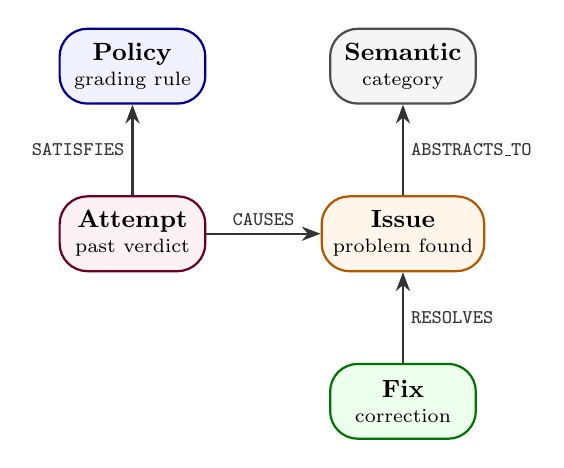
\begin{tikzpicture}[
  font=\small,
  gnode/.style={draw, rounded corners=10pt, align=center, inner sep=4pt,
                minimum height=0.95cm, minimum width=1.85cm, thick},
  rel/.style={-{Stealth[length=2.4mm]}, thick, gray!40!black},
  rlab/.style={font=\scriptsize\ttfamily, fill=white, inner sep=1.5pt}
]
\node[gnode, draw=blue!55!black,   fill=blue!6]
  (policy)  {\textbf{Policy}\\[-2pt]{\scriptsize grading rule}};
\node[gnode, draw=purple!55!black, fill=purple!6, below=1.15cm of policy]
  (attempt) {\textbf{Attempt}\\[-2pt]{\scriptsize past verdict}};
\node[gnode, draw=orange!70!black, fill=orange!8, right=1.45cm of attempt]
  (issue)   {\textbf{Issue}\\[-2pt]{\scriptsize problem found}};
\node[gnode, draw=gray!60!black,   fill=gray!8, above=1.15cm of issue]
  (semantic){\textbf{Semantic}\\[-2pt]{\scriptsize category}};
\node[gnode, draw=green!45!black,  fill=green!7, below=1.15cm of issue]
  (fix)     {\textbf{Fix}\\[-2pt]{\scriptsize correction}};
\draw[rel] (attempt) -- node[rlab, left=1pt]  {SATISFIES}     (policy);
\draw[rel] (attempt) -- node[rlab, above=1pt] {CAUSES}        (issue);
\draw[rel] (fix)     -- node[rlab, right=1pt] {RESOLVES}      (issue);
\draw[rel] (issue)   -- node[rlab, right=1pt] {ABSTRACTS\_TO} (semantic);
\end{tikzpicture}
\caption{The typed memory graph. Each judged item produces an Attempt linked to its Policy; extracted Issues, their Fixes, and abstract Semantic categories structure the judge's past experience. Every node carries a text embedding for similarity retrieval.}
\label{fig:schema}
\end{figure}

\paragraph{Memory-assisted judge (MAJ).} A single-pass judge whose prompt is conditioned on three retrieval stages: (i) similar past attempts, split into passing and failing sets for a contrastive signal; (ii) similar past issues; (iii) recurring issue categories. The similarity thresholds are asymmetric (positive $\ge 0.85$, negative $\ge 0.92$); they were set heuristically during development, and \S\ref{sec:analysis} shows the asymmetry has a measurable consequence.

\paragraph{Exploratory MCTS components.} \emph{MCTS-Judge} decomposes one evaluation into 5--7 generated subtasks and searches over reasoning trajectories with UCT plus an LLM self-assessment. \emph{MCTS-Retrieval} replaces the fixed pipeline with tree search over seven graph retrieval actions, four of them multi-hop. Crossing memory and search gives the ablation modes: \emph{Stateless}, \emph{MAJ}, \emph{MCTS-Judge}, and \emph{MCTS-Judge+Memory}.

\section{Leakage-Free Protocol and the Frozen-Memory Audit}
\label{sec:protocol}

\subsection{Two leakage channels}

The benchmark (\S\ref{sec:setup}) is paired: every question appears twice, once with a passing response and once with a failing one. That pairing creates two accidental leakage paths. \textbf{Paired-item leakage}: split the data by row and one version of a question can land in memory while its twin lands in the test set; when the judge retrieves the twin, it is effectively shown the answer. \textbf{Write-back leakage}: update memory during testing and the verdict on an early item becomes retrievable while scoring a later, related one. Either channel inflates accuracy with zero improvement in judging.

\subsection{Protocol}

Two rules. \textbf{Split by question, not by row}: unique questions are shuffled with a fixed seed and divided in half, and both versions of a question stay on the same side. \textbf{Freeze memory}: memory is built once, before evaluation, and is read-only during the test.

\subsection{The two-layer audit}

A stated freeze is a claim, not a proof. We require the proof, per run (Figure~\ref{fig:audit}).

\begin{figure}[t]
\centering
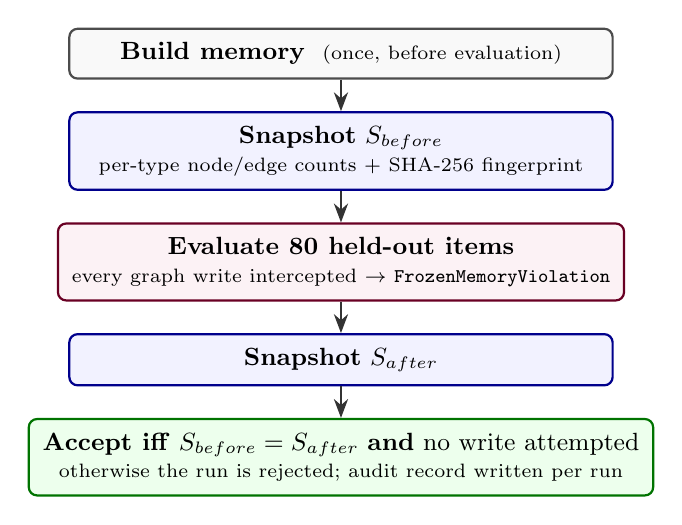
\begin{tikzpicture}[
  font=\small,
  astep/.style={draw, rounded corners=3pt, align=center, inner sep=5pt,
               minimum width=6.9cm, thick},
  rel/.style={-{Stealth[length=2.4mm]}, thick, gray!40!black},
  node distance=0.4cm
]
\node[astep, draw=gray!60!black, fill=gray!5] (build)
  {\textbf{Build memory} \ {\scriptsize(once, before evaluation)}};
\node[astep, draw=blue!55!black, fill=blue!5, below=of build] (before)
  {\textbf{Snapshot} $S_{\text{before}}$\\[-1pt]
   {\scriptsize per-type node/edge counts + SHA-256 fingerprint}};
\node[astep, draw=purple!55!black, fill=purple!5, below=of before] (eval)
  {\textbf{Evaluate 80 held-out items}\\[-1pt]
   {\scriptsize every graph write intercepted $\rightarrow$ \texttt{FrozenMemoryViolation}}};
\node[astep, draw=blue!55!black, fill=blue!5, below=of eval] (after)
  {\textbf{Snapshot} $S_{\text{after}}$};
\node[astep, draw=green!45!black, fill=green!7, below=of after] (verdict)
  {\textbf{Accept iff} $S_{\text{before}} = S_{\text{after}}$ \textbf{and} no write attempted\\[-1pt]
   {\scriptsize otherwise the run is rejected; audit record written per run}};
\draw[rel] (build)  -- (before);
\draw[rel] (before) -- (eval);
\draw[rel] (eval)   -- (after);
\draw[rel] (after)  -- (verdict);
\end{tikzpicture}
\caption{The two-layer frozen-memory audit. Layer 1 (snapshots) detects any mutation after the fact; layer 2 (write interception) prevents it during the run. A run is accepted only if both layers pass.}
\label{fig:audit}
\end{figure}

\textbf{Layer 1, after the fact:} immediately before and after evaluation, take a deterministic snapshot of the graph: per-type node and edge counts, plus a SHA-256 fingerprint over the full stored state (every node's identifier, labels, and complete property map, embeddings included, and every edge triple with its properties). An in-place property edit, not only a node or edge change, alters the fingerprint. Accept the run only if the counts and fingerprints match exactly. The before/after record is written to a per-run audit file.

\textbf{Layer 2, during the run:} patch the write methods of the graph interface with guards that raise \texttt{FrozenMemoryViolation}, and swap the underlying database driver for a read-only proxy that rejects raw Cypher containing write clauses, so holding the driver handle does not bypass the freeze. A violation aborts the entire run; it is never downgraded to an item-level error. The clause filter is syntactic and serves as defense in depth; the state fingerprint remains the authoritative detector.

\textbf{The audit caught a real defect.} On its first application to MCTS-Judge+Memory it failed: the graph grew from 412 to 492 nodes and 831 to 1003 edges, because our own evaluation path was writing each just-judged test item back into memory. That is exactly the write-back leakage the protocol exists to prevent, found in our own code. We fixed it with a read-only evaluation mode; every number below has a passing audit record. A released mutation-test suite exercises the audit against a live database: an in-place property flip and a topology edit issued through raw Cypher both change the fingerprint; wrapper-level and driver-level writes under the freeze both raise; and an attempted write aborts an audited run rather than being recorded as an item error. All tests pass at the released commit. Note the audit cannot be steered toward a desired outcome: its verdict is a hash comparison and an exception, it was built before the audited results were generated, and its first action was to fail on our own code.

\subsection{Memory provenance conditions}

Four conditions isolate where memory comes from and how good it is: \textbf{no-memory} (empty graph); \textbf{self-written} (the judge's own verdicts, reasoning, issues, and fixes from the memory-building half; this is how memory grows in deployment, errors included); \textbf{oracle} (ground-truth labels stored directly, guaranteed correct); and \textbf{poisoned} (oracle memory with a deterministic 10/20/50\% of labels flipped).

\section{Experimental Setup}
\label{sec:setup}

\paragraph{Dataset.} EvalsBench \citep{evalsbench2024} is an open benchmark (Apache-2.0) of 160 graded question--answer pairs over 80 unique questions in the startup and financial-analysis domain. Each row has a topic, question, grading rubric, candidate response, and a balanced pass/fail target (80/80). Each question appears exactly twice, with one passing and one failing response, which makes the benchmark a natural stress test for paired-item leakage. Under the protocol, 40 questions (80 samples) build memory and 40 questions (80 samples) are the held-out test set, seed 42 unless stated. The exact dataset file hash, access date, license, and environment versions are recorded in Appendix~\ref{app:config}.

\paragraph{Judge and search budget.} The judge is GPT-4o, pinned to a fixed API version; all per-sample inputs, verdicts, splits, prompts, retrieval logs, and audit records are released at repository commit \texttt{4787e06f4c28},\footnote{\url{https://github.com/khushpatel1102/maj-research}} so every statistic is re-derivable without re-querying the model. MCTS modes use two rollouts at maximum depth three; a sweep to four rollouts and depth five changed nothing at $4\times$ the cost. All decision extraction uses schema-validated structured outputs \citep{pydantic2024}; an earlier regex extractor failed silently on 15--20\% of responses, a fault that can be mistaken for an empirical finding.

\paragraph{Statistics.} Headline accuracies carry question-clustered bootstrap 95\% CIs (questions resampled with replacement, both paired items moving together); item-level Wilson 95\% intervals \citep{wilson1927} are similar and slightly narrower, and are used where noted. Mode comparisons are paired on identical items, with the exact McNemar test \citep{mcnemar1947} and a paired bootstrap 95\% CI (10{,}000 resamples) \citep{bootstrap1993}; we call a difference significant only if $p<0.05$ \emph{and} the bootstrap interval excludes zero. This joint rule is conservative with respect to multiple comparisons; we apply no further correction because every primary comparison already fails to reject, and a correction only strengthens that conclusion. Observed effects are also small on a standardized scale (Cohen's $h \approx 0.1$ for the largest clean-memory delta). Samples that still fail after exponential-backoff retries are recorded with a null verdict and excluded, with the completed $n$ reported. This detail is material: \S\ref{sec:poisoning} shows it is the difference between the true result and a spurious headline finding.

\section{Results}
\label{sec:results}

\subsection{The motivating observation}

Before the protocol existed, we measured the system conventionally: memory updated during evaluation, paired questions not separated. Memory appeared to help substantially: gains of 6--10 points across capable judge models, and seeding memory with ground-truth examples appeared to lift cold-start accuracy from 78\% to 91\%. We did not retain per-sample logs for these runs, so we report them only as the motivating observation. Several of these configurations interleaved memory-building with evaluation and did not separate paired questions, exposing them to evaluation leakage; \S\ref{sec:channels} decomposes the two structurally isolatable channels and finds that neither alone reproduces the gain, so we attribute it to the compound leak of the original interleaved protocol and/or sampling noise rather than to a single clean channel.

\subsection{Clean-memory comparison}

\begin{table}[t]
\centering
\small
\begin{tabular}{lccc}
\toprule
Mode & Acc.\ [95\% CI] & $n$ & Lat. \\
\midrule
Stateless & 70.0 [62.5, 77.5] & 80 & 3.6\,s \\
MAJ (self-written) & 65.0 [57.5, 72.5] & 80 & 4.5\,s \\
MCTS-Judge & 70.0 [60.0, 80.0] & 80 & 31.8\,s \\
MCTS-J.+Mem. & 71.8 [63.7, 79.7] & 78 & 33.3\,s \\
\bottomrule
\end{tabular}
\caption{Clean-memory results under the leakage-free, audited protocol (GPT-4o, held-out $n{=}80$). CIs are question-clustered bootstrap 95\% intervals (both items of a question resampled together). Coverage: 80/80 for single-pass modes, 78/80 for MCTS-J.+Mem.; under either extreme imputation of the missing outputs no conclusion changes (Limitations).}
\label{tab:clean}
\end{table}

Table~\ref{tab:clean} shows the central result: no configuration outperforms the stateless baseline. MAJ vs.\ stateless is $-5.0$ points (bootstrap CI $[-12.5, +1.3]$, McNemar $p{=}0.29$); MCTS-Judge vs.\ stateless is exactly $0.0$; MCTS-Judge+Memory vs.\ stateless is $+1.8$ ($p{=}0.80$). Every confidence interval in Table~\ref{tab:clean} overlaps the baseline; every paired difference crosses zero (Figure~\ref{fig:deltas}). The 6--10 point gain from the conventional protocol is gone. We changed the measurement, not the system.

\subsection{A response-length shortcut}
\label{sec:length}

Response length alone is a strong predictor on this benchmark: a single length threshold chosen on the memory half scores 75.0\% on the held-out half (longer responses pass), and the stateless judge's verdicts correlate with length (point-biserial $r{=}0.27$). No configuration we tested, memory-augmented or not, beats this superficial baseline; length bias in LLM judges and shortcut artifacts in benchmarks are both well documented \citep{dubois2024length, gururangan2018annotation}. This puts the absolute accuracies in context; the paper's claims rest on the paired mode-versus-mode comparisons, not on absolute levels.

\begin{figure}[t]
\centering
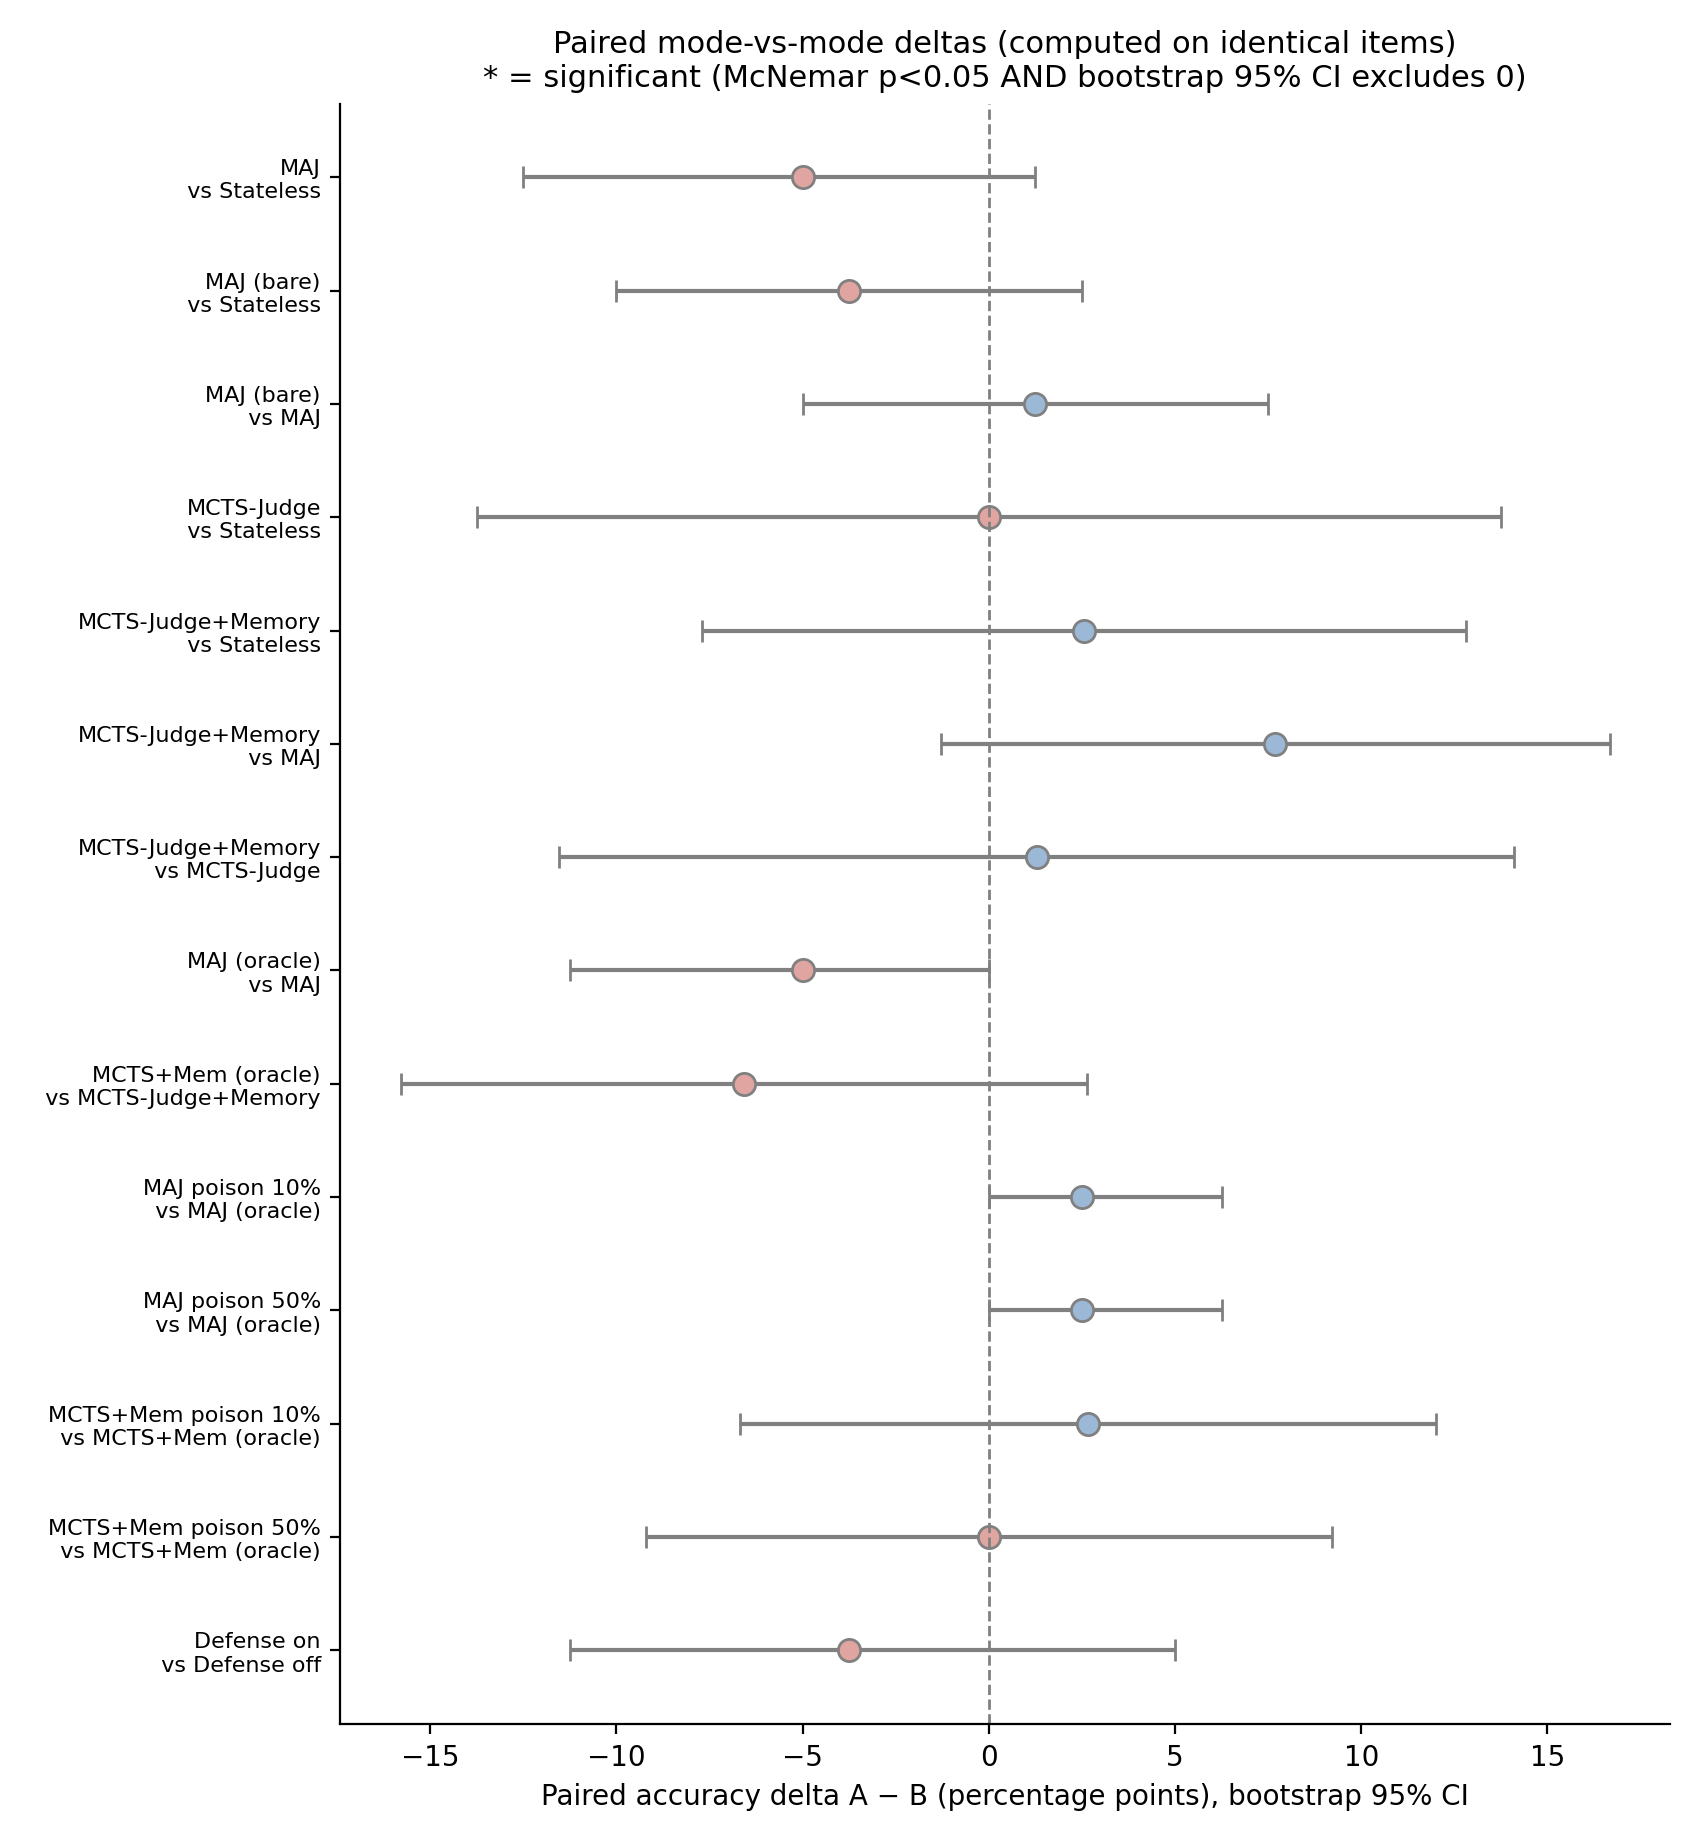
\includegraphics[width=0.72\linewidth]{figures/paired_deltas.png}
\caption{Paired mode-versus-mode accuracy differences with bootstrap 95\% CIs; every clean-memory interval crosses zero.}
\label{fig:deltas}
\end{figure}

\subsection{Oracle memory, schema ablation, seeds}

We attempt to recover the effect in three ways; none succeeds, and each failure is informative.

\textbf{Provenance.} If the gain is masked by noisy self-written labels, perfectly correct oracle labels should recover it: instead, MAJ drops to 60.0\% ($-5.0$, $p{=}0.22$) and MCTS-Judge+Memory to 65.4\% ($-6.6$, $p{=}0.27$). If this retriever--prompt--judge combination were exploiting retrieved labels as evidence, perfect labels should help; they do not. This shows the deployed pipeline does not exploit label correctness, not that the memory carries no information in principle. \textbf{Structure.} If the typed schema carries the signal, removing it should hurt: instead, a bare memory with only Policy and Attempt nodes scores 66.2\% [55.4, 75.7], indistinguishable from the full schema (65.0\%) and from stateless (70.0\%). The Issue/Fix/Semantic extraction does not earn its complexity here. \textbf{Seeds.} To rule out a split artifact, we re-ran on two further seeds: across seeds 42/123/7, stateless scores 70.0/70.0/67.5 and MAJ 65.0/67.5/66.2; the cross-seed range of a single mode ($\approx$5 points) is wider than any mode-vs-mode gap on a single seed. The small differences we see are sampling noise.


\subsection{The poisoning artifact}
\label{sec:poisoning}

\begin{table}[t]
\centering
\small
\begin{tabular}{lcc}
\toprule
Poison rate & MAJ & MCTS-J.+Mem. \\
\midrule
0\% (oracle) & 60.0 & 65.4 \\
10\% & 62.5 & 67.5 \\
20\% & 63.7 & 69.7 \\
50\% & 62.5 & 65.4 \\
\bottomrule
\end{tabular}
\caption{Accuracy (\%) under label poisoning, audited harness. Neither mode degrades; for MCTS-Judge+Memory, 50\% vs.\ oracle is a paired $\Delta$ of exactly $0.0$ ($p{=}1.00$).}
\label{tab:poison}
\end{table}

Our earlier, un-audited harness reported that MCTS-Judge+Memory collapsed to 21.2\% at 50\% poisoning, a 49-point drop large enough to serve as a headline finding. Inspection of the per-sample logs showed otherwise: a mid-run network outage had caused a block of samples to error, and the original code scored every errored sample as a wrong answer. With retries and null-verdict exclusion, the same condition scores 65.4\%, identical to oracle (Table~\ref{tab:poison}). The ``poisoning collapse'' was a property of the harness, not the system. A spurious fragility is the same failure mode as a spurious gain; both originated in the measurement.

\subsection{Bracketing the null: can the judge use memory at all?}
\label{sec:controls}

Table~\ref{tab:baselines} maps each run series to its stateless baseline and the sections that use it. The experiments in this and the following two subsections are a later, independent run, so their stateless baseline is 66.2--68.1\% rather than the 70.0\% of the primary series.

\begin{table}[t]
\centering
\small
\begin{tabular}{lcl}
\toprule
Run series & Stateless & Used in \\
\midrule
Primary audited series (seed 42) & 70.0 & clean memory, ablations, poisoning (\S\ref{sec:results}) \\
Later instrumented run (seed 42) & 66.2 & controls (\S\ref{sec:controls}), $2\times2$ (\S\ref{sec:channels}), \S\ref{sec:flips} thresholds \\
Grouped five-fold CV & 68.1 & cross-validation (\S\ref{sec:cv}), all 160 items \\
\bottomrule
\end{tabular}
\caption{Which stateless baseline belongs to which experiment series. Baselines differ by run inside the documented cross-seed band; every claim is a paired comparison within one series, never across series.}
\label{tab:baselines}
\end{table} That $\approx4$-point drift is expected rather than anomalous: it sits inside the $\approx5$-point cross-seed band reported in \S\ref{sec:results}. The baseline varies by a few points between runs, and so does every mode measured against it, which is why each comparison below is a \emph{paired} test on identical items rather than a difference of two headline numbers.

A null result invites an uninteresting explanation: perhaps the judge simply cannot read retrieved memory, so \emph{no} memory content would ever move its verdict. We rule this out with a memory-use control experiment. Holding the prompt template fixed, we replace the retrieved block with (i) an \emph{answer-injection positive control}: the test item's own ground-truth verdict injected as an exemplar; and three negative controls: (ii) a random unrelated attempt, (iii) label-shuffled exemplars, and (iv) a topically irrelevant block token-matched to the injected block. All four route through the identical memory prompt, so any accuracy change is attributable to the injected content alone.

\begin{table}[t]
\centering
\small
\begin{tabular}{lccc}
\toprule
Injected memory & Acc. & Fail-rec. & Flip\% \\
\midrule
Stateless (none) & 66.2 & 35.0 & -- \\
\textbf{Answer injection} & \textbf{78.8} & \textbf{60.0} & 15.0 \\
Random context & 65.0 & 32.5 & 3.8 \\
Label-shuffled & 63.7 & 30.0 & 2.5 \\
Irrelevant (len-matched) & 68.8 & 40.0 & 5.0 \\
\bottomrule
\end{tabular}
\caption{Memory-use controls (GPT-4o, $n{=}80$). Informative memory lifts accuracy $+12.5$ points, almost entirely on failing items; three uninformative controls sit at the stateless baseline. Flip\% is the fraction of verdicts changed relative to stateless.}
\label{tab:controls}
\end{table}

\begin{figure}[t]
\centering
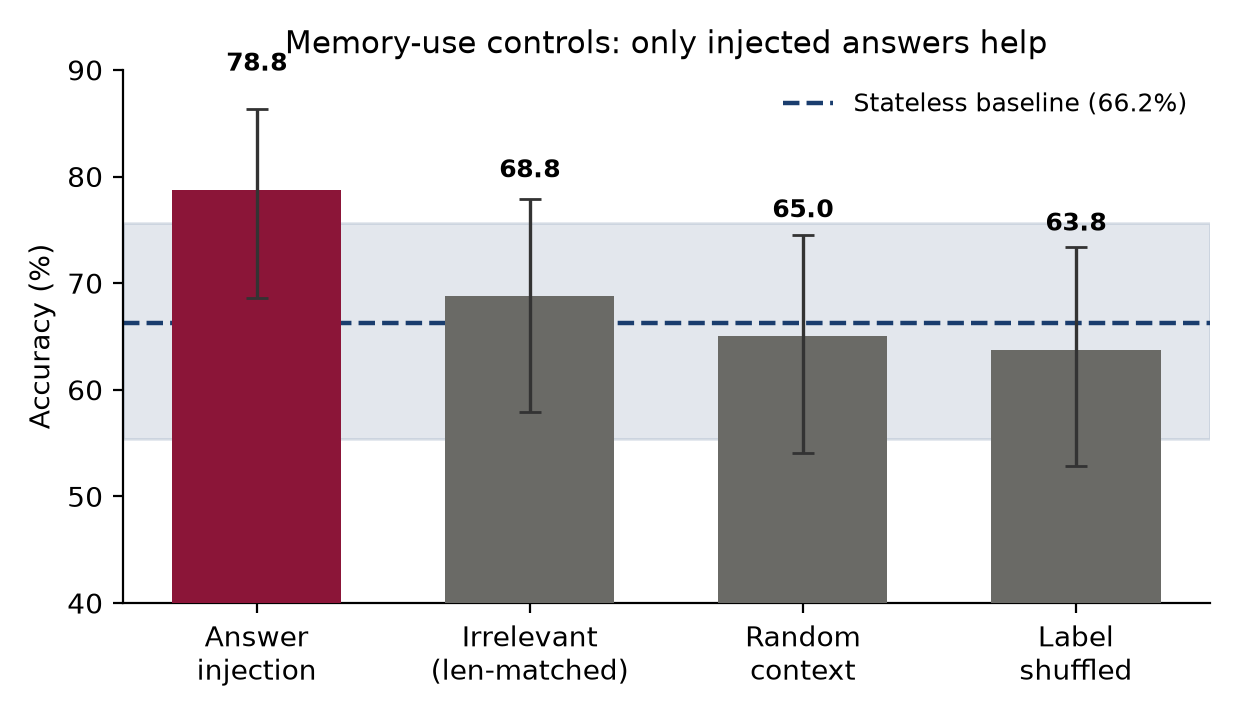
\includegraphics[width=0.86\linewidth]{figures/memory_controls.png}
\caption{Memory-use controls. Only the answer-injection control (informative memory) clears the stateless baseline band; the three uninformative controls fall inside it. Bars are accuracy with Wilson 95\% CIs; the shaded band is the stateless CI.}
\label{fig:controls}
\end{figure}

Table~\ref{tab:controls} and Figure~\ref{fig:controls} show a clean dissociation. When memory carries the answer, accuracy rises $+12.5$ points, concentrated on failing items (fail-recall $35\to60$); per item, the injected answer flips eleven verdicts from wrong to right and only one the other way. The three uninformative controls sit within $2.5$ points of the no-memory baseline (question-clustered 90\% CIs on the paired deltas: $[-5.0,+2.5]$, $[-5.0,0.0]$, $[-1.3,+6.2]$); a formal equivalence test at a $\pm5$-point margin is inconclusive at $n{=}80$, so we claim consistency with no effect, not demonstrated equivalence. \emph{The judge can use memory when memory is informative}; the null elsewhere is therefore a property of the benchmark's memory carrying no verdict-relevant signal, not of a memory-blind judge. This is the positive half of the bracket that Proposition~\ref{prop:bayes} predicts: accuracy moves exactly when the injected content changes $P(Y\mid X,M)$, and not otherwise.

\subsection{Cross-validated reliability}
\label{sec:cv}

To confirm the null is not an artifact of a single 80-item split, we run five-fold grouped cross-validation at the question level (every one of the 160 items is a held-out test item in exactly one fold; memory is built on the other four folds), for the four primary modes only. Confidence intervals come from a question-cluster bootstrap that resamples questions, keeping each pass/fail pair together.

\begin{table}[t]
\centering
\small
\begin{tabular}{lcc}
\toprule
Mode & Acc. & $\Delta$ vs.\ stateless [95\% CI] \\
\midrule
Stateless & 68.1 & -- \\
MAJ (self) & 68.8 & $+0.6$ $[-3.8, +5.0]$ \\
MAJ (oracle) & 64.4 & $-3.7$ $[-7.5, 0.0]$ \\
MAJ (balanced) & 68.1 & $\phantom{+}0.0$ $[-4.4, +4.4]$ \\
\bottomrule
\end{tabular}
\caption{Grouped five-fold cross-validation over all $n{=}160$ items, question-cluster bootstrap CIs. No mode significantly beats stateless; oracle memory trends slightly worse. The balanced-minus-self contrast is $-0.6$ $[-3.1, +1.3]$.}
\label{tab:cv}
\end{table}

Table~\ref{tab:cv} confirms the null at double the sample size: MAJ with self-written memory is $+0.6$ points with a CI spanning zero, and oracle memory does not help (its CI touches zero from below, the most direct evidence that the memory carries no exploitable label signal). This is the negative half of the bracket, and it is now cross-validated rather than resting on one split.

\subsection{Isolating the leakage channels}
\label{sec:channels}

The motivating observation (\S\ref{sec:results}) attributed the conventional $+6$--$10$ point gain to evaluation leakage. To test which channel is responsible, we cross the two structurally isolatable channels in a $2\times2$: split by question (twins together) versus by row (twins may separate, the paired-item channel), and memory frozen versus written back during evaluation (the write-back channel).

\begin{table}[t]
\centering
\small
\begin{tabular}{lcc}
\toprule
Cell & Bal.\ acc. & $\Delta$ vs.\ clean \\
\midrule
Question $\times$ frozen (clean) & 66.2 & -- \\
Row $\times$ frozen (paired-item) & 63.4 & $-2.9$ \\
Question $\times$ write-back & 67.5 & $+1.2$ \\
Row $\times$ write-back (both) & 66.8 & $+0.5$ \\
\bottomrule
\end{tabular}
\caption{$2\times2$ leakage decomposition (GPT-4o, $n{=}80$, balanced accuracy to neutralize the row split's $44/36$ class imbalance). Deltas are computed from unrounded accuracies. Neither isolated channel reproduces the conventional gain.}
\label{tab:channels}
\end{table}

The result (Table~\ref{tab:channels}) is instructive and contrary to our initial expectation: \emph{neither structurally isolatable channel reproduces the conventional gain}. Paired-item leakage moves balanced accuracy $-2.9$ points (the larger raw drop is mostly the $44/36$ class imbalance the row split induces), and write-back alone is $+1.2$. We therefore do not claim the conventional gain was manufactured by these two clean channels. The most consistent explanation is that the original observation arose under a protocol that interleaved memory-building with evaluation, a stronger compound leak than either channel in isolation, and/or was inflated by sampling noise. What survives is the operational point the paper is built on: the apparent gain does not survive any clean, audited re-measurement.

\subsection{Reliability harness}

Accuracy is one number; three further probes characterize the judge along other axes. \emph{Stochastic stability}: judge the same item twice and stateless agrees with itself 94\%, MAJ 95\%, MCTS-Judge+Memory 90\%. \emph{Label-flip discrimination}: rewrite a response to invert its ground truth and verdicts flip correctly 65--70\% of the time, similarly across modes. \emph{Defense filter}: a similarity-threshold filter on retrieval under 50\%-poisoned memory does not help (65.0\% vs.\ 64.8\%), an honest negative for that defense. The stability numbers matter below: a judge that already agrees with itself 90--95\% of the time leaves memory very little noise to correct.

\section{Analysis: Why Memory Neither Helped nor Harmed}
\label{sec:analysis}

A null result is only useful if it is explained: what did memory actually do to individual verdicts, why is that the expected behavior, and what design change would escape it?

\subsection{Verdict-flip decomposition}
\label{sec:flips}

\begin{table}[t]
\centering
\small
\begin{tabular}{lcccc}
\toprule
Pair (A vs.\ B) & agree & $b$ & $c$ & $\to$pass \\
\midrule
Stateless / MAJ & 90.0\% & 2 & 6 & 6/8 \\
Stateless / MCTS-J.+M. & 79.5\% & 9 & 7 & 6/16 \\
MAJ self / MAJ oracle & 92.5\% & 1 & 5 & 5/6 \\
MAJ full / MAJ bare & 91.2\% & 4 & 3 & 3/7 \\
\bottomrule
\end{tabular}
\caption{Paired verdict-flip decomposition on identical items ($n{=}80$; $n{=}78$ for the MCTS comparison, whose two null-verdict items are excluded). \emph{agree}: identical verdicts; $b$: items B fixes (A wrong, B right); $c$: items B breaks; $\to$pass: fraction of all changed verdicts that moved toward ``pass''.}
\label{tab:flips}
\end{table}

Every mode judged the identical items, so the effect of memory can be read item by item (Table~\ref{tab:flips}). Three facts emerge.

\textbf{(1) Memory is mostly inert.} MAJ agrees with the stateless verdict on 90\% of items. Swapping self-written memory for oracle changes 7.5\% of verdicts. Deleting three of the five node types changes 8.8\%. The retrieved context block occupies roughly half the prompt and moves almost nothing; the verdict is dominated by the judge's own reading of the task, rubric, and response.

\textbf{(2) The verdicts memory does move follow the judge's bias, not the truth.} For MAJ vs.\ stateless, all six harmful flips turned a correct ``fail'' into a wrong ``pass,'' both helpful flips went the other way, and six of eight flips moved toward ``pass.'' The class-conditional numbers sharpen the picture: every mode is far better on passing items than failing ones (stateless 97.5\% vs.\ 42.5\%), and attaching memory makes the asymmetry \emph{worse} (MAJ: 97.5\% vs.\ 32.5\%). Oracle memory shows the same signature (five of six flips toward pass). Memory here acts as a mild leniency anchor: retrieved passing exemplars tend to prime the judge toward ``pass'' on the hard failing items where it was already weakest. A candidate cause is the asymmetric retrieval thresholds of \S\ref{sec:system} (positive $\ge 0.85$, negative $\ge 0.92$), which admit more passing than failing exemplars. We tested this directly: symmetric thresholds do admit more failing exemplars (mean negatives per item $2.01\to2.71$), confirming the mechanism is real, but the accuracy consequence is small, a $+2.5$ point fail-recall recovery (one item in forty) that merely returns balanced MAJ to the stateless baseline, and the cross-validated balanced-minus-self contrast is a reliable zero ($-0.6$ $[-3.1, +1.3]$, \S\ref{sec:cv}). We therefore report the tilt as present in the retrieved context but with an accuracy cost at the edge of detectability at this scale, rather than as a confirmed driver of the null.

\textbf{(3) Structured reasoning partially de-anchors.} MCTS-Judge+Memory is the only memory mode whose flips are net-positive ($b{=}9$ vs.\ $c{=}7$), and it shifts the class balance the other way (94.9\% pass / 48.7\% fail): eight of its nine fixes converted false passes into correct fails. Forcing the judge to score 5--7 rubric-specific subtasks before aggregating dampens the holistic leniency prior, consistent with the anchoring account, though the net effect remains insignificant.

\subsection{What memory can contribute, in principle}
\label{sec:theory}

Let $X$ be the stateless input (task, rubric, response), $Y \in \{\text{pass},\text{fail}\}$ the label, and $M$ the retrieved memory. The quantity of interest is the accuracy of the \emph{Bayes-optimal} decision rule, which for any available conditioning information $Z$ predicts $\arg\max_y P(Y{=}y \mid Z)$ and attains accuracy $A^*(Z) = \mathbb{E}_Z\!\left[\max_y P(Y{=}y \mid Z)\right]$. Comparing the stateless conditioning $X$ to the memory-augmented conditioning $(X,M)$:

\begin{proposition}[Bayes value of side information; classical]
\label{prop:bayes}
Assume $(X, M, Y)$ has a well-defined joint distribution and that $A^*$ is evaluated under its true conditionals. Then $A^*(X,M) \ge A^*(X)$, and the gain is governed by how much the posterior moves when $M$ is revealed:
\[
A^*(X,M) - A^*(X) \;=\; \mathbb{E}_{X,M}\!\big[\max_y P(Y{=}y\mid X,M)\big] - \mathbb{E}_{X}\!\big[\max_y P(Y{=}y\mid X)\big],
\]
with equality if and only if, for almost every $(X,M)$, some class that is most probable given $X$ alone remains most probable given $(X,M)$; in particular, equality holds whenever $Y \perp M \mid X$.
\end{proposition}

This is a standard consequence of the comparison of statistical experiments \citep{blackwell1951, blackwell1953}; we state it for orientation, not as a new result. In words: memory can raise the \emph{achievable} accuracy only to the extent that the conditional label distribution given $(X,M)$ differs from the one given $X$ alone; if memory is conditionally uninformative about the label, the Bayes-optimal accuracy is unchanged regardless of the decision rule.

\emph{Is $M$ conditionally informative here?} The protocol is built to make $P(Y\mid X,M)\approx P(Y\mid X)$: the question-level split guarantees no retrieved item concerns the test question, the rubric is fully specified inside $X$, and graded financial QA sits within GPT-4o's parametric competence, so a neighboring question's verdict shifts the posterior negligibly. The oracle experiment probes this: if the deployed judge extracted label evidence from retrieved memory, oracle memory should raise its accuracy; instead it is worth nothing ($-5.0$ and $-6.6$ points, n.s.). This shows that \emph{this} retriever, prompt, and judge do not exploit the information; it does not establish that the memory carries none, and a different pipeline might exploit signal this one ignores.

\emph{A separate, smaller channel: realized-judge noise.} The proposition bounds the \emph{Bayes-optimal} accuracy. The judge we actually deploy is a stochastic rule $f$, not the Bayes rule, so conditioning on $M$ could in principle also help by stabilizing $f$ toward its own posterior even when $A^*$ is unchanged. We do not claim memory cannot help through this route; we report only that the room for it is small here. The stability probes (\S\ref{sec:flips} context) show the judge disagrees with itself on just 5--10\% of items, so the realized judge already sits close to a deterministic rule, and any stabilizer, memory or otherwise, has at most that 5--10\% of verdicts to move. Self-disagreement is thus a \emph{diagnostic} for how much stochastic instability exists to be corrected, not a bound on all conceivable benefit of memory.

A descriptive accounting identity re-expresses the realized accuracy change in terms of how often memory changes a verdict and how often those changes are corrective (it attributes no mechanism):
\[
\mathbb{E}[\Delta] \;=\; \underbrace{P(\text{flip})}_{0.10 \text{ for MAJ}} \cdot \bigl(2q - 1\bigr), \quad q = P(\text{flip corrective}),
\]
and the decomposition in \S\ref{sec:flips} measures $q = 2/8$ for MAJ. When $M$ does not move the posterior (\S\ref{sec:theory}), the flips that do occur are driven by the stylistic content of $M$ (here, the exemplar imbalance) rather than by label evidence, so $q$ falls below $1/2$ and memory mildly hurts, in the direction of the judge's prior bias. Substituting the measured values gives $0.10 \times (2 \cdot 0.25 - 1) = -5.0$ points, recovering the observed MAJ delta by construction. Read descriptively, the same identity locates where the conventional-protocol illusion lives: leakage makes $P(Y\mid X,M)$ depend sharply on $M$ (the paired item's verdict is now in memory), pushes $q$ far above $1/2$, and manufactures the 6--10 point ``gain.''

\subsection{Practical remedies, and when memory should help}
\label{sec:remedies}

The account above is constructive; it identifies the available levers.

\paragraph{(a) Balance the contrastive signal.} The leniency tilt is a property of the retrieval design, not of memory per se. Symmetric thresholds, or enforcing equal numbers of passing and failing exemplars in the context block, remove the systematic push toward ``pass'' that produced MAJ's $-5.0$. This is a minimal, directly testable change.

\paragraph{(b) Gate memory by informativeness.} $\mathbb{E}[\Delta]$ is negative whenever $q<1/2$, so memory should be injected only when retrieval is likely to be evidential, e.g.\ when the top retrieved attempt is a near-duplicate of the current item, falling back to the stateless judge otherwise. Gating bounds the harm at zero by construction and preserves the benefit on recurring items, the one regime where $P(Y\mid X,M)$ genuinely departs from $P(Y\mid X)$.

\paragraph{(c) Use memory at the population level.} The judge's dominant failure is a stable class bias (42.5\% on failing items), and a store of past evaluations is the data needed to \emph{measure} that bias per Semantic category. Instead of injecting instance-level exemplars, let memory supply a calibration correction: a per-category decision-threshold shift estimated from stored (verdict, outcome) pairs. This converts the graph from an ineffective evidence channel into a statistically well-grounded bias-correction channel, and it is the use we consider most promising.

\paragraph{(d) Target regimes where memory moves the posterior.} Proposition~\ref{prop:bayes} predicts memory helps when the judge cannot already solve the task from $X$: weaker judge models with headroom below the rubric, a regime in which model size demonstrably changes capability on knowledge-engineering tasks \citep{heim2025scaling}; domains whose verdicts depend on conventions the model has never seen (project-specific style guides, private grading norms); workloads with recurring or near-duplicate items. These are falsifiable predictions. They also mark the boundary of our claim: the result is ``no effect for GPT-4o on this benchmark,'' not ``memory never helps,'' and our data do not support the latter.

\section{Conclusion}

We asked when persistent memory helps an LLM judge, and we required an answer whose measurement could be independently checked. The protocol (question-level partition, frozen memory, a two-layer cryptographic audit) verifies per run that the stored memory state did not change, and it caught a real leakage defect in our own code on its first application. Under this protocol the answer, for GPT-4o on this benchmark, is that no benefit is measurable: neither memory nor tree search outperforms the stateless judge, and an apparent 6--10 point gain did not survive audited re-measurement, and an apparent poisoning collapse was traced directly to a harness defect. The per-item analysis supports a simple reading: under the leakage-free protocol memory appears to move the conditional label distribution very little, so the Bayes-achievable gain is small, while the separate route of stabilizing the stochastic judge has only its 5--10\% self-disagreement to exploit; the few verdicts memory does change skew toward ``pass,'' consistent with a leniency-anchoring account; rebalancing the retrieval removes the skew's proximate cause without a reliable accuracy change. The general lesson is that both the promise and the fragility of judge memory, as commonly measured, are properties of the harness: trustworthy claims about memory-augmented judging require audited measurement first. We release the protocol, audit, per-sample records, and a one-command reproduction script so the practice can be adopted directly.

\section*{Limitations}

\textbf{Power.} $n{=}80$ gives a minimum detectable effect of roughly 12--15 points: sufficient to test the conventional protocol's 6--10 point claim, which it refutes, but not to exclude a genuine effect of a few points. We therefore state the result as ``no effect detected at this scale.'' \textbf{Single judge, single benchmark.} All audited results use GPT-4o on graded financial QA; \S\ref{sec:remedies}(d) states explicitly where we expect the picture to change. \textbf{Excluded samples.} At most four samples per configuration errored after retries and were excluded; under either extreme imputation (all excluded scored wrong, or all scored right) every affected accuracy moves by at most $2.5$ points and no significance conclusion changes. \textbf{Poisoning pattern.} We tested uniform random label flips only; structured adversarial poisoning may behave differently. \textbf{Conventional-protocol numbers.} Their per-sample logs were not retained, so they are reported as a motivating observation, not a verified claim. \textbf{Audit scope.} The audit verifies the absence of the two channels we model (mutation of the stored graph during evaluation, paired-item splitting); its guards are in-process and its Cypher filter is syntactic, so adversarial evasion or out-of-band database access is out of scope. The runs reported here were audited with the v1 topology-scope fingerprint, which suffices for the two modeled channels because both manifest as node and edge additions (write-back inserts new Attempt and Policy nodes, and no evaluation code path edits properties in place), but would not have caught an in-place property edit; the released v2 fingerprint hashes the full stored state and passes the mutation-test suite.

\section*{Acknowledgments}
This work was carried out at Innopolis University. We thank the EvalsBench authors for the open benchmark.

\bibliography{references}

\appendix

\section{Audit Record Format}
Each run emits a machine-readable record holding the before/after snapshots (per-type node and relationship counts, total counts, and a SHA-256 fingerprint: v2 hashes the full stored state including all node properties; the v1 records for the reported runs hash node identifiers and edge triples) and their diff. A run is leakage-free only if the diff is empty and the fingerprints match; records are released with the code.

\section{The Assembled Memory Prompt}
\label{app:prompt}

The retrieved memory block below is the exact structure produced by the retrieval pipeline (excerpts shortened). It is prepended to the task, rubric, and candidate response; the anti-anchoring warning at the top is part of the published prompt. Despite occupying roughly half the prompt, this block changes only 10\% of verdicts (\S\ref{sec:flips}).

\begin{quote}\small\ttfamily
IMPORTANT: These are REFERENCE examples only. Each case is UNIQUE.\\
Do NOT assume this case will have the same outcome as similar past cases.\\
Judge THIS response on its OWN merits against the grading criteria.\\[4pt]
SUCCESSFUL EXAMPLES (similar responses that passed):\\
\ 1. [similarity: 91\%] Response excerpt: ``DCF projects future cash flows at a stage-appropriate discount rate...''\\
\ \ \ \ Why it passed: ``covers all three methods, names the discount-rate trade-off.''\\[4pt]
FAILED EXAMPLES (similar responses that failed - check if same issue applies):\\
\ 1. [similarity: 93\%] Response excerpt: ``Pre-money valuation is the value of the company before investment...''\\
\ \ \ \ Why it failed: ``tautological; never names a method.''\\[4pt]
PAST ISSUES (only flag if SPECIFICALLY present in this response):\\
\ 1. [similarity: 91\%] ``missed discount-rate justification''\\[4pt]
PATTERNS TO CHECK (warnings only - NOT automatic failures):\\
\ 1. incomplete-methodology [similarity: 90\%]
\end{quote}

The leniency mechanism of \S\ref{sec:flips} is visible in this structure: the passing exemplars clear the lower 0.85 threshold more often than failing exemplars clear 0.92, so the block above typically contains more ``successful'' than ``failed'' entries.

\section{Experiment--Artifact Manifest}
\label{app:manifest}

All artifacts live at repository commit \texttt{4787e06f4c28}.

\begin{table}[h]
\centering
\small
\begin{tabular}{lll}
\toprule
Experiment & Driver script & Per-item records / audits \\
\midrule
Primary series (clean, oracle, poison) & \texttt{benchmark\_leakage\_free.py} & \texttt{results/leakage\_free\_*, lf\_*} + \texttt{*\_audit.json} \\
Multi-seed replication & same, \texttt{--seed} & \texttt{results/lf\_*\_seed\{7,123\}*} \\
Memory-use controls & \texttt{experiments/exp2\_memory\_controls.py} & \texttt{results/exp2\_*} \\
$2\times2$ leakage decomposition & \texttt{experiments/exp1\_2x2\_leakage.py} & \texttt{results/exp1\_*} (+dose logs) \\
Grouped five-fold CV & \texttt{experiments/exp3\_grouped\_cv.py} & \texttt{results/exp3\_cv\_*} \\
Threshold (leniency) test & \texttt{experiments/exp4\_leniency\_anchor.py} & \texttt{results/exp4\_*} (retrieval logs) \\
Length / equivalence / sensitivity & \texttt{experiments/round3\_analyses.py} & \texttt{results/round3\_analyses.json} \\
Audit mutation tests & \texttt{tests/test\_audit\_mutation.py} & 7/7 passing at the commit above \\
\bottomrule
\end{tabular}
\caption{Map from every reported experiment to its driver script and released artifacts. Splits are reproduced by seed (Appendix~\ref{app:config}); prompts are in \texttt{src/prompts.py}.}
\label{tab:manifest}
\end{table}

\section{Configuration}
\label{app:config}

\begin{table}[h]
\centering
\small
\begin{tabular}{ll}
\toprule
Parameter & Value \\
\midrule
Judge model & GPT-4o (pinned API version) \\
Graph store & Neo4j Community server 5.x (June runs); 5.26.28 (verification env); Python driver \texttt{neo4j} 5.15.0 \\
Dataset file & \texttt{benchmark\_df.csv}, SHA-256 \texttt{84886f73\ldots0c76}, obtained 2026-02, Apache-2.0 \\
Embeddings & text-embedding-ada-002, 1536-d, HNSW index \\
Retrieval top-$k$ & attempts 3 (per class), issues 5, semantic patterns 3 \\
Similarity thresholds & positive $\ge0.85$; negative $\ge0.92$; issues $\ge0.90$ \\
Negative-exemplar cap & at most $|\text{positives}|+1$ \\
Symmetric (balanced) variant & both attempt thresholds $0.85$ \\
MCTS budget & 2 rollouts, max depth 3 \\
Transient-error handling & 5 retries, exponential backoff; then null verdict, excluded \\
Sampling temperature & default (primary series); $0$ (control and instrumented runs) \\
Splits / seeds & question-level 40/40; seeds 42, 123, 7; CV: 5 question-level folds \\
Statistics & Wilson 95\% CI; exact McNemar; paired bootstrap, $10{,}000$ resamples \\
\bottomrule
\end{tabular}
\caption{Complete configuration. Per-item retrieval logs for the instrumented runs (pre- and post-threshold exemplar counts, per-exemplar similarities, top-1 retrieved label, memory token counts) are included in the released per-sample records. The temperature row records a deliberate difference: the later control and instrumented experiments pin temperature to $0$ so that verdict flips measure the effect of memory content rather than sampling noise; the primary series uses the published judge unchanged.}
\label{tab:config}
\end{table}

\end{document}
